%!TEX TS-program = lualatex
%!TEX encoding = UTF-8 Unicode

\documentclass[hyphens,11pt,a4paper]{article}
\usepackage[top=2.5cm, bottom=2.5cm, left=3cm, right=2cm,includefoot]{geometry}
%\usepackage[margin=2.5cm,includefoot]{geometry}
\usepackage[portuges]{babel}
\usepackage[T1]{fontenc}
\usepackage{lipsum}
\usepackage{url}

\usepackage{fontspec}
\defaultfontfeatures{Mapping=tex-text}
\setmainfont{Verdana}

\usepackage{setspace}

\renewcommand{\baselinestretch}{1}
\setlength{\parskip}{.5cm}
\setlength{\parindent}{1.25cm}


\usepackage{titlesec}
\titleformat*{\section}{\normalsize\bfseries}
\titleformat*{\subsection}{\normalsize\bfseries}
%\titleformat*{\subsubsection}{\large\bfseries}

\titlespacing*{\section}{0pt}{10pt}{-10pt}
\titlespacing*{\subsection}{0pt}{10pt}{-10pt}

\usepackage{indentfirst}

\usepackage{hyperref}
\usepackage[hyphenbreaks]{breakurl}
\usepackage[alf,abnt-full-initials=yes,abnt-last-names=abnt]{abntex2cite}

\newcommand{\alc}{\ensuremath{\mathcal{ALC}}}
\newcommand{\dland}{\sqcap}         % concept intersection
\newcommand{\dlor}{\sqcup}       % concept union
\newcommand{\subs}{\sqsubseteq}  % concept subsumption
\newcommand{\conc}{\textit}         % concept name
\newcommand{\role}{\textit}         % role name
\newcommand{\pspace}{\textsc{PSpace}}



\def\seq{\rightarrow }
\def\De{\ensuremath{\mathcal{D}}}
\def\d{\ensuremath{\Pi}}
\def\F{\ensuremath{\mathcal{F\;}}}
\def\L{\ensuremath{\mathcal{L}}}
\def\fe#1{\ensuremath{\mathcal{F_{#1}}}}
\def\N{\ensuremath{\mathcal{N}}}
\def\CC{\ensuremath{\mathcal{C}}}
\def\EF{$e$-$\mathcal{F}\;$}
\def\SF{$\mathcal{SF}$}
\def\SS{\ensuremath{\mathscr{S}}}
\def\={\ensuremath{\mathrel{\mathop:}=}}


\def\dfrac{\displaystyle\frac}
\def\A#1#2{\ensuremath{\bigwedge\limits_{{#1} = 0}^{#2}}}
\def\B#1#2{\ensuremath{\bigvee\limits_{{#1} = 0}^{#2}}}
\def\C#1#2#3{\ensuremath{\bigvee\limits_{0\leq {#1} < {#2} \leq{#3}}}}
\def\D#1#2#3{\ensuremath{\bigwedge\limits_{0\leq {#1} < {#2} \leq{#3}}}}
\def\SEQ#1#2{\ensuremath{#1_1,\ldots ,#1_{#2}}}
\def\S#1#2{\ensuremath{(A_{#1}\rightarrow A_{#2}})}
\def\SE#1#2#3{\ensuremath{[A_{#1}\rightarrow A_{#2}}]^{#3}}


\begin{document}
\pagestyle{empty}
\begin{center}
{\bf Uso de ontologia para projeto e desenvolvimento de software baseado em framework } 
\end{center}

\begin{flushright}
Luiz Gustavo Dias\footnote{Universidade Federal de Goiás- Mestrado Profissional em Gestão Organizacional.\\ gusttavodiias@gmail.com}\\[.01cm]
Vaston Gonçalves da Costa\footnote{Universidade Federal de Goiás- Unidade Acadêmica Especial de Matemática e Tecnologia.\\ vaston@ufg.br}
\end {flushright}

{\footnotesize
\noindent{\bf Resumo}: Gerenciamento de conhecimento é uma disciplina que emprega métodos para aumentar a competitividade de empresas. Em suma, o gerenciamento de conhecimento trata o conhecimento existente de uma matéria de forma a que possam inferir informações úteis para o desenvolvimento de ações. Ao contrário de métodos exploratórios, uma abordagem formal que visa inferir informações consistentes do conhecimento necessita de uma base lógica correta e completa. Neste sentido que o uso de técnicas advindas da lógica descritiva vem se mostrando bem aceita. Neste trabalho se apresenta uma abordagem baseada em lógica descritiva para auxiliar na extração de conhecimento de uma ontologia voltada para o gerenciamento de habilidades.
\\[.2cm]
\noindent{\bf Palavra-chave}: Representação do conhecimento. lógica descritiva. Gerenciamento de habilidades. }

\section*{Introdução}

O conhecimento das competências e habilidades das pessoas que prestam serviço a uma empresa (sejam do quadro da empresa, ou que prestem serviço eventual) é o recurso mais importante de qualquer empreendimento. Pois, permite gerenciar, dentre outras coisas, uma melhor tomada de decisão, planejar estratégias ou propor novas abordagens para problemas. 

Gerenciar o conhecimento das habilidades dos recursos humanos de uma empresa não pode ser relegado a poucas pessoas de um departamento de pessoal~\cite{}. É necessário  estabelecer uma base de dados que agregue todas as informações das pessoas que podem ser úteis no desenvolvimento da companhia, isto é, capacidade, experiência, áreas de conhecimento.

Representar todo o conhecimento das habilidades de pessoas pode contribuir para expor falhas que precisam ser tratadas e os níveis de competências de cada uma. O que, permite planejar contratações, buscar pela melhor abordagem para qualificar o quadro e, bem como, definir o crescimento na carreira dentro da empresa (plano de cargos).

Computacionalmente, representação e explicação do conhecimento é uma parte da área da inteligência artificial que se preocupa em como um agente usa o que é conhecido para decidir o que fazer. Isto é, representação e explicação do conhecimento é o estudo do pensamento como um processo computacional~\cite{brachman2004knowledge}.

%A pesquisa em lógica e em representação do conhecimento tem uma forte conexão com o desenvolvimento da área de Teoria da Computação na sua vertente estrutural. Na última década do século passado a vertente estrutural e a algorítmica estão se relacionando mais fortemente com a lógica matemática via Teoria da Prova e Teoria de Modelos Finitos. 

Do ponto de vista prático, pode-se citar um grande interesse atual em lógica de descrição (DL \emph{description logic}) no desenvolvimento da chamada Web Semântica, onde enormes bases de conhecimento, de procedências diversas, estarão disponíveis na rede para serem consultadas e manipuladas por agentes inteligentes de \emph{software}. De fato a linguagem OWL (\emph{Web Ontology Language}) fornece a DL uma sintaxe ao estilo XML, visando a integração destas lógicas com as ferramentas e os formalismos mais comuns da WWW; satisfeitas certas restrições, uma ontologia escrita em OWL correspondente exatamente a uma teoria em DL.


O uso de DL e seus mecanismos de inferências se mostram adequados para os mais variados empregos na área de representação de conhecimento pois são capazes de compreender diferentes formas nas quais pode se representar o conhecimento e de retirar conclusões a partir das informações encontradas~\cite{AOW07}.


\section{Desenvolvimento}
No contexto de gestão do conhecimento é sabido que o uso de fragmentos de lógica de primeira ordem é bem recebido como base lógica para a representação e manipulação de conhecimento e sua análise formal, em particular o fragmento decidível de primeira ordem de uma lógica de descrição (DL), \alc.

Especificamente, em DL termos de conceitos descrevem classes de indivíduos em algum universo, enquanto termos de papéis (também chamados de propriedades) representam relações binárias ligando indivíduos. Em \alc, a sintaxe de conceitos e propriedades é definida pela gramática
%$C,D \to \bot \mid \top \mid A \mid  \neg C \mid C \dland D \mid C \dlor D \mid \forall R.C \mid \exists R.C$
\[ 
		\begin{array}{rcll} 
			C, D  & \to    & A             & \textrm{(conceito atômico)} \\ 
					& \mid   &  \top         & \textrm{(conceito universal)} \\ 
					& \mid   &  \bot         & \textrm{(conceito vazio)} \\ 
					& \mid   &  \neg C       & \textrm{(negação)} \\ 
					& \mid   &  C \dland D   & \textrm{(interseção)} \\ 
					& \mid   &  C \dlor D    & \textrm{(união)} \\ 
					& \mid   &  \forall R.C  & \textrm{(restrição de valor)} \\ 
					& \mid   &  \exists R.C  & \textrm{(quantificação existencial)} \\
		\end{array} 
\] 
		 sendo que $A$ representa o conceito atômico e $R$ representa os nomes atômicos de papéis (o único tipo de termo de papel). 
		 Uma das maneiras usuais de interpretar termos de conceitos consiste em traduzi-los para expressões de teoria dos conjuntos. 
		
		Formalmente, define-se uma interpretação como sendo um mapeamento $\mathcal{I}$ de termos de conceitos para conjuntos de indivíduos de um universo $\Delta$ e de termos de papéis para relações binárias sobre $\Delta$, que satisfazem as seguintes condições:
%\begin{singlespace}
\begin{small}		
		\[
		 \begin{array}{rcl}
				\mathcal{I}(\top)             & = & \Delta   \\
				\mathcal{I}(\bot)             & = & \emptyset \\
				\mathcal{I}(\neg C)           & = & \Delta - \mathcal{I}(C) \\
				\mathcal{I}(C \dland D)    & = & \mathcal{I}(C) \cap \mathcal{I}(D)  \\
				\mathcal{I}(C \dlor D)     & = & \mathcal{I}(C) \cup \mathcal{I}(D)  \\
				\mathcal{I}(\forall R.C)   & = & \{ a \in \Delta \mid \forall b. [(a,b) \in 
																												\mathcal{I}(R) \Rightarrow b \in \mathcal{I}(C)] \}   \\
				\mathcal{I}(\exists R.C)   & = & \{ a \in \Delta \mid \exists b. [(a,b) \in 
																												\mathcal{I}(R) \land b \in \mathcal{I}(C)] \}   \\
		 \end{array}
		\]
\end{small}
%\end{singlespace}
Se um indivíduo $a$ pertence ao conjunto representado por um termo de conceito $C$, dizemos que $a$ \emph{está em} $C$. Se um par $(a, b)$ de indivíduos pertence à relação binária representada por $R$, dizemos que $b$ \emph{preenche a propriedade $R$ de} $a$, ou que $b$ \emph{é um preenchedor de} $R$. 

		Informalmente, um termo de conceito da forma $\forall R.C$ representa o conjunto de todos os indivíduos que possuem todos os preenchedores de $R$ (caso existam) em $C$. Um termo de conceito da forma $\exists R.C$ representa o conjunto de todos os indivíduos que possuem pelo menos um preenchedor de $R$ em $C$.

		Em DL, uma fórmula de \emph{subsunção}, escrita $C \subs D$, representa o enunciado de que a classe denotada por $C$ está contida na classe denotada por $D$. Uma fórmula de \emph{equivalência} $C \equiv D$ representa o enunciado de que $C$ subsume $D$ e $D$ subsume $C$; ou seja, $C$ e $D$ denotam a mesma classe. 
		Uma \emph{TBox} (de \emph{terminologia}) é uma coleção de fórmulas de subsunção e/ou equivalência em DL tomadas como axiomas. Em outras palavras, uma \emph{TBox} é uma \emph{teoria} na linguagem de DL. O processo de \emph{inferência} ou  \emph{dedução} consiste em descobrir que fórmulas de DL são consequências lógicas de uma \emph{TBox} $T$. 

	Definimos uma {\it ontologia} (cf. ~\cite{Gruber} ) como simplesmente uma DL \emph{TBox}.  O uso mais comum de uma ontologia é o de armazenar uma taxinomia de termos em um certo domínio de conhecimento. Do ponto de vista de uma DL, esta taxinomia é definida por meio de \emph{hereditariedade}, que é exatamente a relação de subsunção entre termos. Os termos e propriedades em uma ontologia podem ser caracterizados por meio de uma fórmula em DL.
	 %
	 Ontologias são usualmente  expressas em OWL ({\it Web Ontology Language}) (cf.~\cite{Dean}). OWL tem uma sublinguagem (OWL DL) cujos construtores coincidem com os permitidos em DL. 

%Um dos autores deste projeto integrou o TECMF, laboratório da PUC-Rio coordenado pelo prof. Edward Hermann Haeusler, para trabalhar no projeto ANUBIS-CTINFO. Este projeto objetiva a solução da gestão de bases de conhecimento para a segurança da informação e buscava o desenvolvimento de uma metodologia de apoio a edição e manutenção de ontologias a partir do texto de padrões de segurança (ditos {\it Frameworks}) via ferramental desenvolvida pela equipe. Além da edição/criação de ontologias a partir de texto, um módulo de análise formal provendo explicações em linguagem natural está em fase final de desenvolvimento. 
%Este módulo é um provedor de explicações para Teoremas (enunciados na forma de subsunção) provados no sistema lógico de cálculo de sequentes. 
%Este é fundamentalmente mais um ganho da Teoria da Prova na área de representação do conhecimento.
%Ele substituiu o raciocinador clássico em Tableaux normalmente utilizado para a lógica de descrição.  
%


%Pretendemos seguir nesta linha com a aplicação de isomorfismos para a extração de conteúdo computacional (explicações) a partir de sistemas de Dedução Natural, pois provas produzidas em dedução natural possuem leitura em forma de algoritmo estruturado, permitindo produzir explicações de forma mais clara.
%
%Também, pretendemos trabalhar com o aperfeiçoamento da ferramenta produzida no projeto ANUBIS-CTINFO. Atualmente estamos trabalhando com um novo módulo de provas automáticas baseado em cálculo de sequentes com lado esquerdo vazio, denotado por $SEQ_0$. Em seguida, investigaremos a acoplação de sequentes no método horizontal visando a compressão de provas. Em um resultado preliminar, conseguimos reduzir de superpolinomial para polinomial o limite superior para provas livres de corte de algumas proposições combinatórias. A partir da validação destes resultados, o objetivo será implementar este novo sistema dedutivo no provador automático de teoremas produzido no projeto ANUBIS-CTINFO.
%
%Como resultado inicial da participação no projeto ANUBIS-CTINFO, conseguimos publicar um artigo no {\it $3^{rd}$ Australasian Ontology Workshop} \cite{AOW07}.

\section{Procedimentos utilizados}

\citeonline{AOW07} propuseram a estrutura de uma ontologia voltada para segurança da Informação tendo como base para sua criação normas e políticas de segurança definidas por consórcios e ISOS.

No âmbito do gerenciamento de habilidades não há uma referência mínima do que deve se conter numa ontologia que lida com habilidades. Pode-se, contudo, citar os trabalhos de \cite{Colucci:jucs_9_12:a_formal_approach_to}
que apresenta uma ontologia que lida com a oferta e demanda de habilidades, como se fosse voltada para um mercado de compra e venda de habilidades. A abordagem baseada em formalização utilizando lógica descritiva e raciocínio, supera correspondência subsunção simples e permite ranking de partida e categorização. A utilização de tais métodos e ferramentas resultam no aumento potencial do know-how de organizações, tornando-as mais competitivas no mercado. A abordagem é capaz de lidar com casos em que não existem combinações perfeitas, ou seja, encontrar esses perfis disponíveis que sejam compatíveis, e vice-versa. Os benefícios abordagem proposta pelos autores, são a possibilidade de explorar a estrutura ontológica para a gestão de competências; a possibilidade de distinção semântica entre o potencial, e resultados parciais entre perfis; e um ranking que está próximo de um que fosse construído a partir do julgamento humano. Os autores finalizam a pesquisa apontando que estavam trabalhando em outro tipo de ontologia, que geraria resultados mais próximos ao raciocínio humano, onde seriam empregados outros recursos computacionais, como algoritmos baseados em grafos bipartidos e algoritmos para alocação de recursos.


Mas, para situações específicas, podem se criar ontologias cada vez mais especialistas. É o caso da proposta de \cite{johnston2013} que buscam mostrar em sua pesquisa a importância da gerência de dados relacionada ao cotidiano universitário. Os autores buscam identificar as habilidades de gerenciamento de dados necessárias para identificar pessoas que são capazes de gerir adequadamente os dados na era digital, e também para que posteriormente se torne possível desenvolver uma metodologia educacional baseada na gerência de dados.  O trabalho foi produzido através de entrevistas realizadas a um grupo de pesquisa composto por quatro estudantes de engenharia e um docente, ambos de uma universidade de Minnesota. A coleta de dados foi realizada levando em consideração a fase de vida dos dados, sendo nomeadas pelos autores como: Dados Brutos, Coleta \& Organização, Processamento/Análise, Compartilhar/Arquivar e Preservação dos dados.

Este estudo possui abordagem qualitativa, uma vez que será apresentada uma análise bibliográfica que visa emergir aspectos subjetivos sobre determinado assunto (Dalfovo, 2008). Para que fosse possível a realização do mesmo, foi necessária a aquisição de material bibliográfico que trabalhasse o tema “Gestão do conhecimento”, para isso foram definidos como diretórios de pesquisa, periódicos de renome como sendo eles: Journal of Professional Issues in Engineering Education and Practice (JPIEEP), International Journal of Project Management (IJPM), Information \& Management (IM), Journal of Universal Computer Science (JUCS).  
%Tais periódicos foram definidos como fontes de pesquisa pela qualidade nos trabalhos publicados e pela importante contribuição no desenvolvimento de pesquisas acerca do tema definido para este trabalho.
%A amostra foi definida por conveniência, sendo composta por 04 artigos que levantam questões relacionadas a Gestão do Conhecimento, publicados entre os anos de 2003 e 2013. 
%A análise dos trabalhos selecionados foi feita levando em consideração três critérios principais: Qual o nível de investimento das empresas em P&D (podendo ser classificados como insatisfatório, regular e alto), Apoio do estado em P&D nas indústrias nacionais (podendo ser classificado como inexistente, insatisfatório, regular ou alto), e Retorno das empresas que investem em pesquisa e desenvolvimento (podendo ser classificado em inexistente, insatisfatório, regular e alto).

Também pode se citar os trabalhos de \cite{wu2004}   \cite{pant2008} \cite{Carbone2004}  que abordam as características necessárias de pessoas para determinadas atividades.

\subsection{Uma ontologia para Gerenciamento de Habilidades}

Antes, cabe lembrar que uma ontologia é mais do que um vocabulário. Seu propósito é: primeiro, armazenar a taxonomia para a representação de habilidades; segundo, armazenar as formas lógicas que conectam as habilidades às necessidades da empresa; terceiro, armazena axiomas de forma a suportar inferências em DL.

\begin{description}
\item Taxonomia 

Além de definir um vocabulário comum que os usuários devem se empenhar em empregar, a ontologia deve ajudar na tarefa de extrair conhecimento de textos em linguagem natural, conforme \cite{Aussenac-Gilles:2005:TAO:1412350.1412354}.

Para auxiliar no processo de extração de conhecimento de textos, cada conceito é associado com seu sinônimo via Wordnet. Na ontologia a associação é realizada via a anotação de propriedade \emph{hasSynSet}.

\item Descrição

Esta parte da ontologia armazena a representação formal das habilidades pessoas e possivelmente a representação formal dos controles associados a habilidade. Isto é, as habilidades podem ser pensadas como \emph{o que deve se ter} enquanto o controle especifica esta ação, isto é, \emph{o que garante se ter}. Por exemplo, pode-se querer um engenheiro com habilidade= experiência e e o controle de experiência para engenheiro=5 anos de experiência em atividade, por exemplo.

\item Axiomas

As equivalências e subsunções necessárias para garantir que sentenças com significados próximos devem ser mapeados a mesma forma lógica.

Por  exemplo,  "Desenvolva X para obter Y" é equivalente à "Obtenha Y" é equivalente á formula em DL:

$\exists hasVerb.(Desenvolva \dland \exists hasTheme.X\dland \exists hasPurpose.Y)\equiv \exists hasVerb.Y$

\end{description}


\section{Discussão e Resultados}
A proposta do trabalho é desenvolver uma ontologia para Gerenciamento de Habilidades. Para tal, deve-se construir assistente de formalização para se evitar o emprego de uma grande quantidade de axiomas para teoria, e se evitar uma taxonomia com redundâncias. 

Além deste assintente, deve-se empregar um raciocinador que permita consultar a base de conhecimento bem como  responda as perguntas realizadas nos conhecimentos da base. Optou-se por empregar o raciocinador Pallet que é gratuito e pode ser acoplado no auxiliar de ontologias Protégè. A figura\ref{figura1} apresenta as etapas necessáiras para a construção da ontologia. 


\begin{figure}[h]
\begin{center}
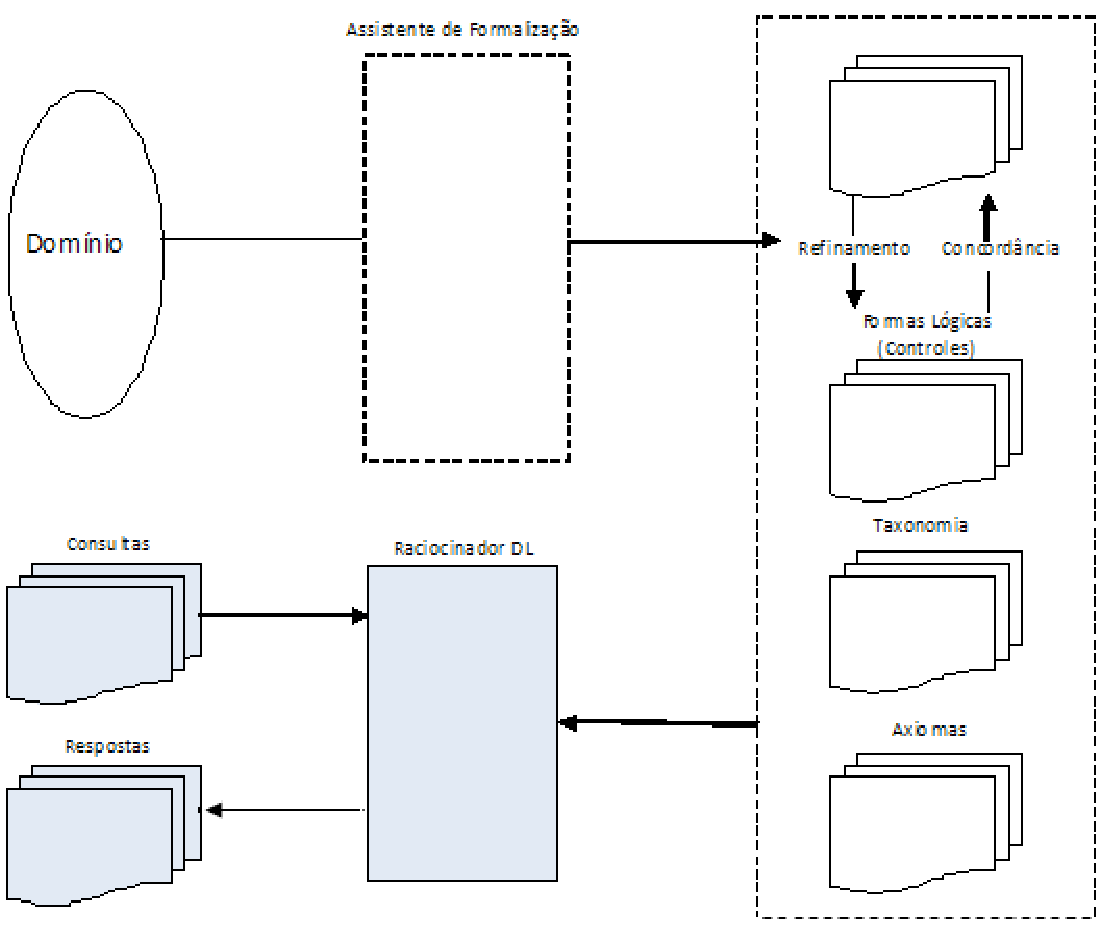
\includegraphics[width=.7\textwidth]{vaston.pdf}
\end{center}
\caption{Elementos de validação da Ontologia para Gerenciamento de Habilidades.\label{figura1}} 
\end{figure}


\section*{Conclusões ou Considerações finais}

O trabalho propõe a construção de uma ontologia que possa auxiliar na representação e extração de conhecimento de bases envolvendo habilidades de pessoas.

Vez que os estudos mostram que as ontologias para tal abordagem variam muito de um perfil de empresa para outro, nesta etapa do trabalho optou-se por criar uma ontologia genérica, baseada no trabalho de \cite{AOW07}, que sirva com um \emph{framework} para uma especialização para negócios específicos.

A próxima etapa consiste em criar uma ontologia específica e aplicar a esta conceitos de inferencia de conhecimento automáticas ou semi-automáticas em um caso real.


%\bibliographystyle{abnt-num}
\bibliography{referencias}

%Nesta seção, que não é numerada, devem constar TODAS as obras e autores que foram citados no corpo do artigo, rigorosamente como estabelece a ABNT (cf. NBR 6023/2002). Os autores são alinhados à esquerda, sem recuo, por ordem alfabética do último nome e, se houver, mais de uma obra do mesmo autor, por ordem cronológica decrescente.



\end{document}  